\chapter{Conjuntos, relaciones y funciones}

\section{Conjuntos}

El concepto de \textit{conjunto} aparece en todos los campos de las Matemáticas,
pero, ¿qué  debe  entenderse  por él? La \textit{Teoría de conjuntos} 
fue introducida por Georg Cantor (1845-1917); desde 1869, Cantor ejerció 
como profesor en la Universidad de Halle y entre 1879 y 1884 publicó una 
serie de seis artículos en el \textit{Mathematische Annalen}, en los 
que hizo una introducción básica a la teoría de conjuntos. En su 
\textit{Beiträge zur Begründung der transfiniten Mengenlehre}, 
Cantor dio la siguiente definición de conjunto:

\begin{figure}[h]
  \centering
  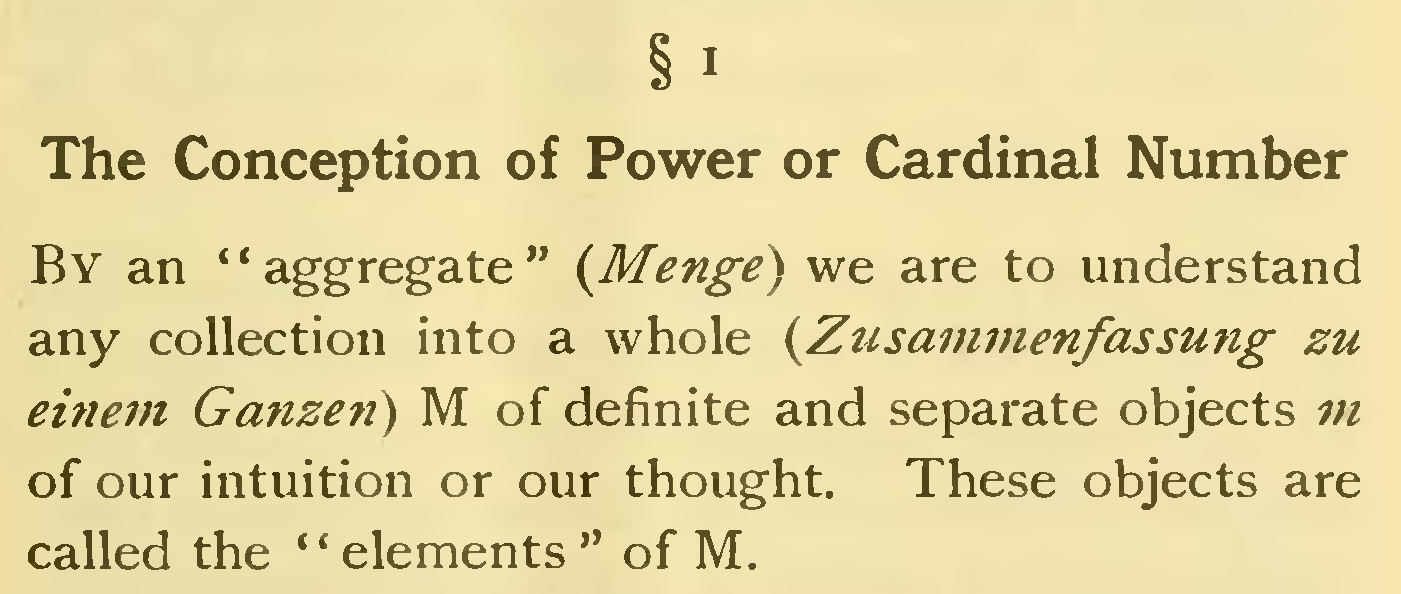
\includegraphics[scale=.2]{fig/definicionConjunto}
  \captionsetup{font=footnotesize}
  \caption{Fragmento del texto traducido al inglés en el que Cantor 
           da la definición de conjunto}
\end{figure}

\begin{center}
    <<Debemos entender por ``conjunto'' (\textit{Menge}) cualquier 
    colección vista como un todo (Zusammenfassung zu einem Ganzen), $M$, 
    de objetos separados y bien definidos, $m$, de nuestra intuición 
    o pensamiento. Estos objetos son los ``elementos'' de $M$>> 
\end{center}

Felix Hausdorff, en 1914, dice: <<un conjunto es una reunión de cosas que 
constituyen una totalidad, es decir, una nueva cosa>>, y añade: 
<<esto puede difícilmente ser una definición, pero sirve como demostración 
expresiva del concepto de conjunto a través de conjuntos sencillos como
el conjunto de habitantes de una ciudad o el de átomos de Hidrógeno del 
Sol>>. 

Un conjunto así definido no tiene que estar compuesto necesariamente
de elementos homogéneos y además, da lugar a cuestiones filosóficas como 
si podemos llamar \textit{conjunto} a aquel que no posee ningún elemento. 
Matemáticamente, conviene aceptar solo elementos que compartan alguna 
propiedad y definir el \textit{conjunto vacío} como aquel que no tiene 
elemento alguno.

El gran mérito de Cantor fue considerar conjuntos \textit{transfinitos} 
(que tiene infinitos elementos), concepto inaudito hasta avanzado el siglo 
XIX, hablar del \textit{cardinal} de un conjunto como el número de sus
elementos y hablar de \textit{conjuntos equivalentes} cuando puede
establecerse una biyección entre ellos; ideas ya apuntadas por Bolzano,
quien se centró demasiado en el aspecto filosófico, sin llegar a formalizar
sus ideas.

A lo largo de la sección, haremos una pequeña introducción a la Teoría de 
Conjuntos, presentando formalmente sus conceptos más importantes.

\begin{comentario}
Referencias:
\begin{itemize}
  \item $https://en.wikipedia.org/wiki/Set_(mathematics)$
  \item $http://catedu.es/materranya/suplemento3.pdf$
  \item $https://rodas5.us.es/file/a774213d-a15a-41df-816c-e633fb1a5876/1/01-Conjuntos.pdf$
  \item Piensa en Haskell (Ejercicios de programación funcional con Haskell)
\end{itemize}

Falta darle formato, organizar e ir añadiendo
\end{comentario}

\entrada{Conjuntos}

\section{Relaciones}

Las relaciones que existen entre personas, números, conjuntos y muchas
otras entidades pueden formalizarse en la idea de relación binaria. En esta 
sección se define y desarrolla este concepto además 

\entrada{Relaciones}

\section{Relaciones homogéneas}

\entrada{RelacionesHomogeneas}

\section{Funciones}

\entrada{Funciones}

%%% Local Variables:
%%% mode: latex
%%% TeX-master: "MD_en_Haskell"
%%% End:
